%!TEX TS-program = pdflatex
%!TEX root = main.tex
%!TEX encoding = UTF-8 Unicode

\section{Tempi}
%Usando \emph{multi\_batch\_plot.Rmd}
I grafici che seguono sono stati generati usando R e \emph{ggplot}.
%I valori usati per H e K sono gli interi tra 1 e 10, fissato un numero di corridoi vengono generati tutti gli input 

\noindent
In \autoref{fig:second_plot} si vede come il tempo totale di risoluzione degli input dati.
Notare come in genere il modello Minizinc sia migliore del modello ASP.
I pallini indicano se il modello è andato in timeout.
L'andamento del grafico è dato dal modo in cui sono stati generati gli input, quindi dal loro ordinamento: durante la generazione venivano effettuati due cicli for annidati uno per il numero di corridoi ed uno per il numero di stanze.
Confrontando \autoref{fig:input_sizes}, \autoref{fig:second_plot} e \autoref{fig:first_plot} si osserva come l'andamento delle dimensioni degli input sia in linea con la complessità dell'istanza, misurata in tempo di risoluzione dei modelli.
In \autoref{fig:first_plot} si può  osservare il tempo di risoluzione dei due modelli.
I pallini indicano per quali istanze i modelli sono andati in timeout.
\begin{figure}[ht]
  \centering
  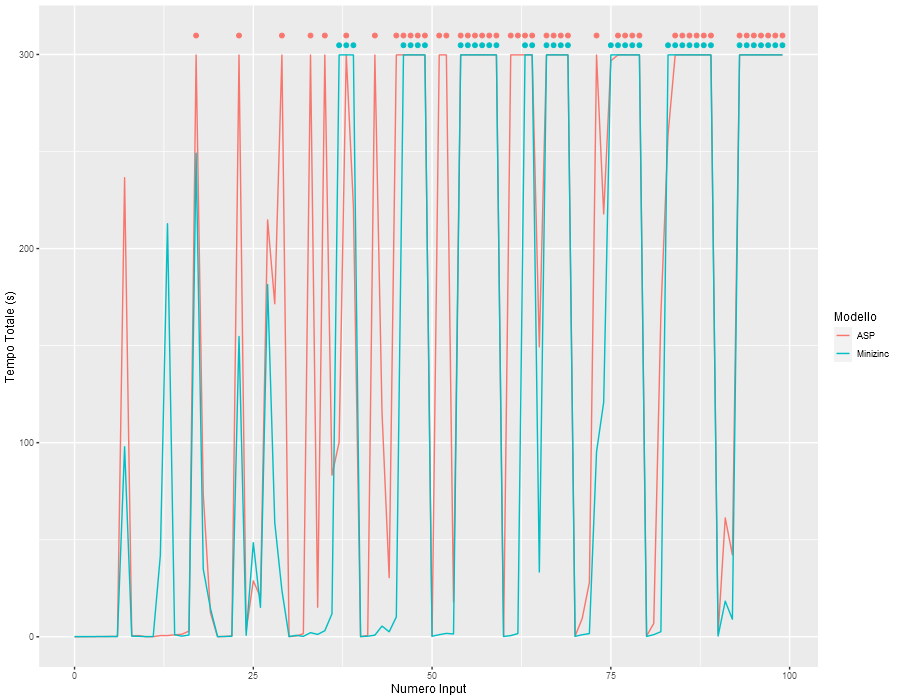
\includegraphics[width=\textwidth]{second_plot}
  \caption{Input in ordine di numerazione}
  \label{fig:second_plot}
\end{figure}
\begin{figure}[ht]
  \centering
  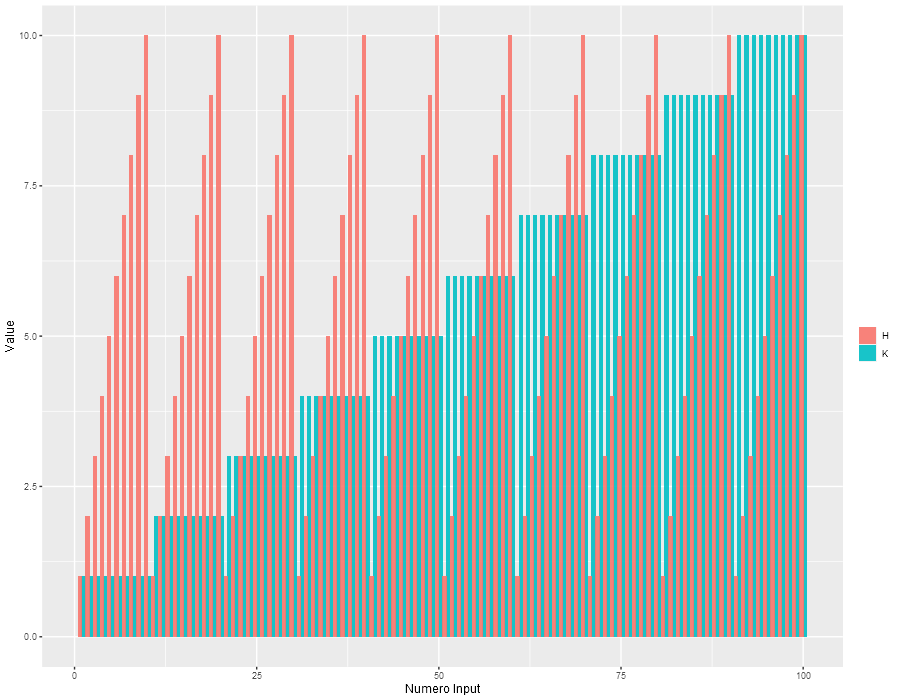
\includegraphics[width=\textwidth]{input_sizes}
  \caption{Dimensioni H e K degli input in ordine di numerazione}
  \label{fig:input_sizes}
\end{figure}

\begin{figure}[ht]
  \centering
  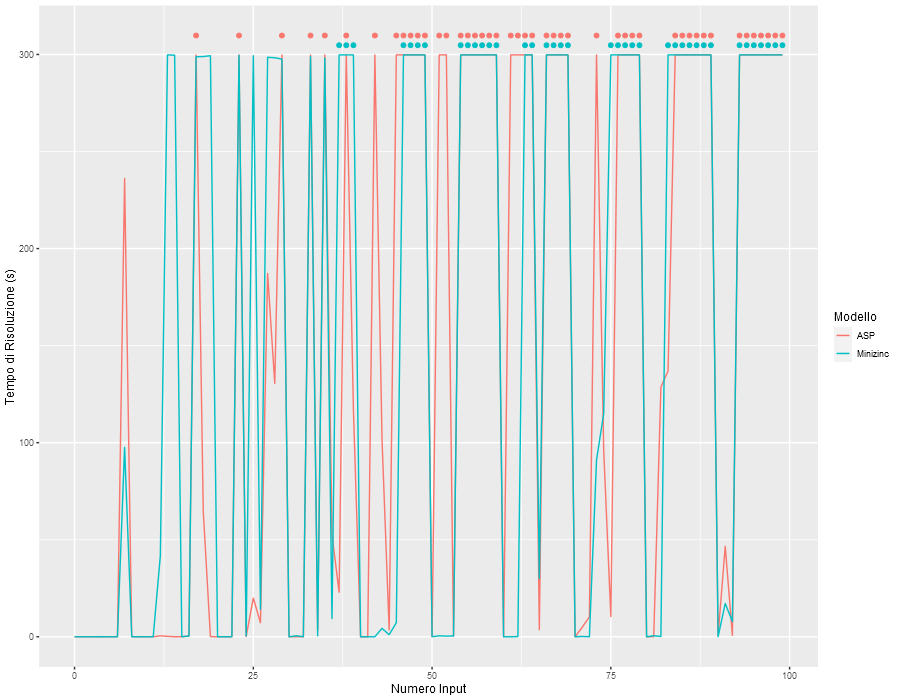
\includegraphics[width=\textwidth]{first_plot}
  \caption{Input in ordine di numerazione}
  \label{fig:first_plot}
\end{figure}
\cleardoublepage

\noindent
Osservando soltanto le soluzioni per le quali non si è raggiunto il timeout ed ordinando secondo tempo totale di risoluzione del modello ASP si ottiene il grafico in \autoref{fig:no_timeout_times}.
\begin{figure}[ht]
  \centering
  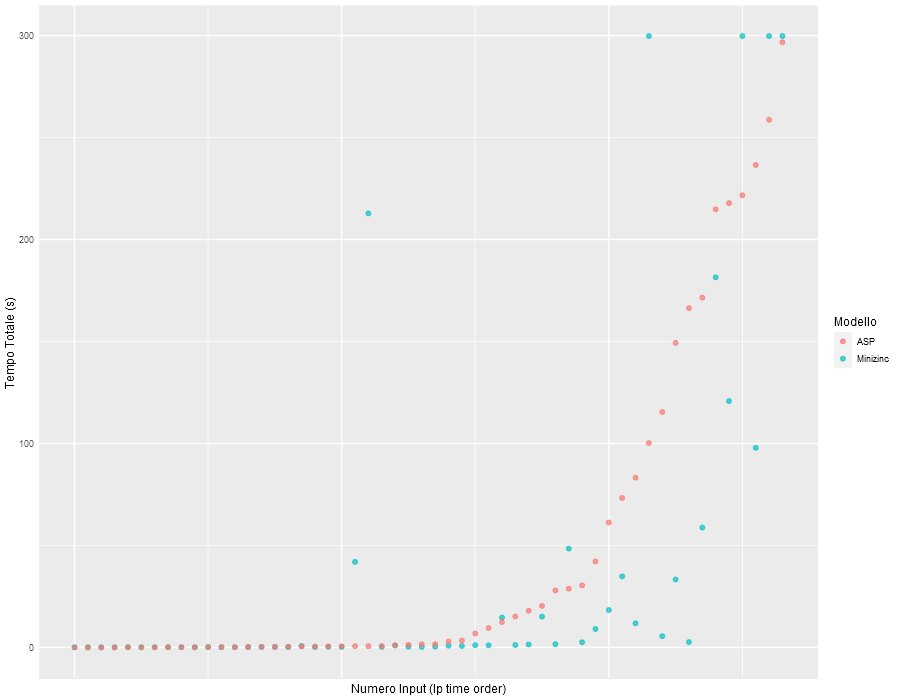
\includegraphics[width=.8\textwidth]{sorted_lp_time_no_timeout_times}
  \caption{Input in ordine crescente di tempo totale per il modello ASP}
  \label{fig:no_timeout_times}
\end{figure}
Notare come in più occasioni, su uno stesso input, un modello performa molto bene mentre l'altro ha difficoltà.
Una delle cause di questo fenomeno è il modo in cui il modello Minizinc cerca le soluzioni, cioè iniziando a collocare gli ospiti in quarantena nelle stane più lontane e dei piani più alti.
Ciò non viene fatto nel modello ASP.
Le osservazioni appena fatte valgono anche per il tempo di risoluzione, come si vede in \autoref{fig:no_timeout_solvetimes}.
\begin{figure}[ht]
  \centering
  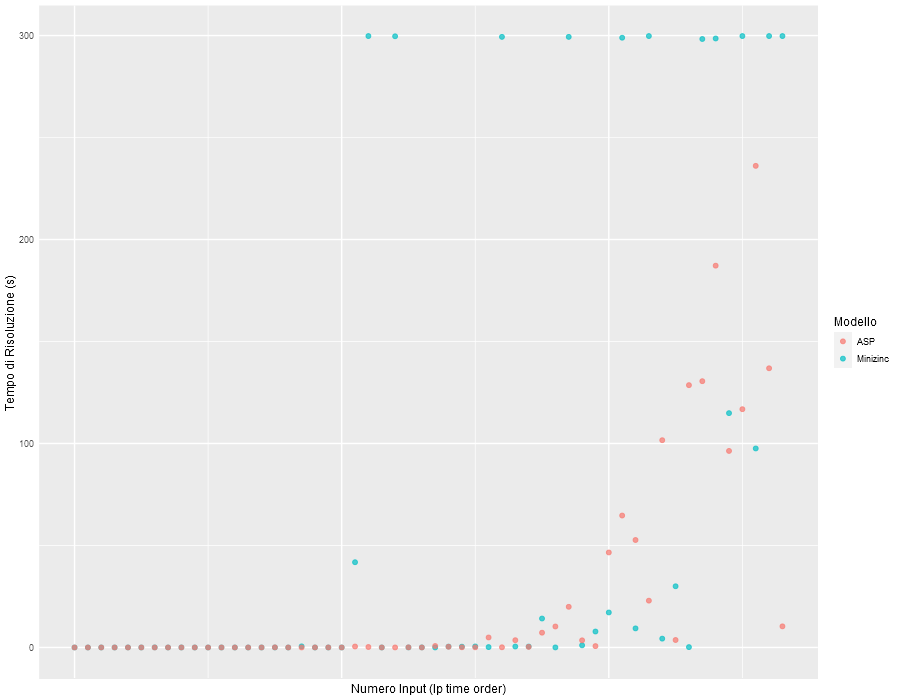
\includegraphics[width=.8\textwidth]{sorted_lp_time_no_timeout_solveTimes}
  \caption{Input in ordine crescente di tempo totale per il modello ASP}
  \label{fig:no_timeout_solvetimes}
\end{figure}

\noindent
Confrontando i valori ottenuti dai due modelli si ha che
\begin{itemize}
  \item Minizinc batte sul tempo complessivo ASP 47 volte su 100;
  \item Minizinc batte sul tempo di risoluzione ASP 30 volte su 100.
\end{itemize}
Possiamo quindi dire che i modelli hanno capacità confrontabili e che il tempo di grounding inficia in modo notevole sulle prestazioni del modello ASP.
Infatti, considerando soltanto i tempi di risoluzione, il modello ASP è da preferirsi.
